\begin{pa} \label{PA:9.6} In this activity we consider how we might use vectors to define a curve in space.
    \ba
    \item On a single set of axes in $\R^2$, draw the vectors $\left\langle \cos(0), \sin(0) \right\rangle$, $\left\langle \cos\left(\frac{\pi}{2}\right), \sin\left(\frac{\pi}{2}\right) \right\rangle$, 
    
     $\left\langle \cos\left(\pi\right), \sin\left(\pi\right) \right\rangle$,  \text{ and } $\left\langle \cos\left(\frac{3\pi}{2}\right), \sin\left(\frac{3\pi}{2}\right) \right\rangle$ with their initial points at the origin.


    \item On the same set of axes, draw the vectors $\left\langle \cos\left(\frac{\pi}{4}\right), \sin\left(\frac{\pi}{4}\right) \right\rangle$, $\left\langle \cos\left(\frac{3\pi}{4}\right), \sin\left(\frac{3\pi}{4}\right) \right\rangle$, 
    
     $\left\langle \cos\left(\frac{5\pi}{4}\right), \sin\left(\frac{5\pi}{4}\right) \right\rangle$,  \text{ and } $\left\langle \cos\left(\frac{7\pi}{4}\right), \sin\left(\frac{7\pi}{4}\right) \right\rangle$ with their initial points at the origin.



   \item Based on the pictures from parts (a) and (b), sketch the set
     of \emph{terminal} points of all of the vectors of the form
     $\langle \cos(t), \sin(t) \rangle$, where $t$ assumes values from
     0 to $2 \pi$. What is the resulting figure? Why?


    \ea

\end{pa} 

\begin{activitySolution}
    \ba
    \item The vectors are shown at left in the figure below. 
  %  \begin{figure}[ht]
      \begin{center}
      \resizebox{!}{2.5in}{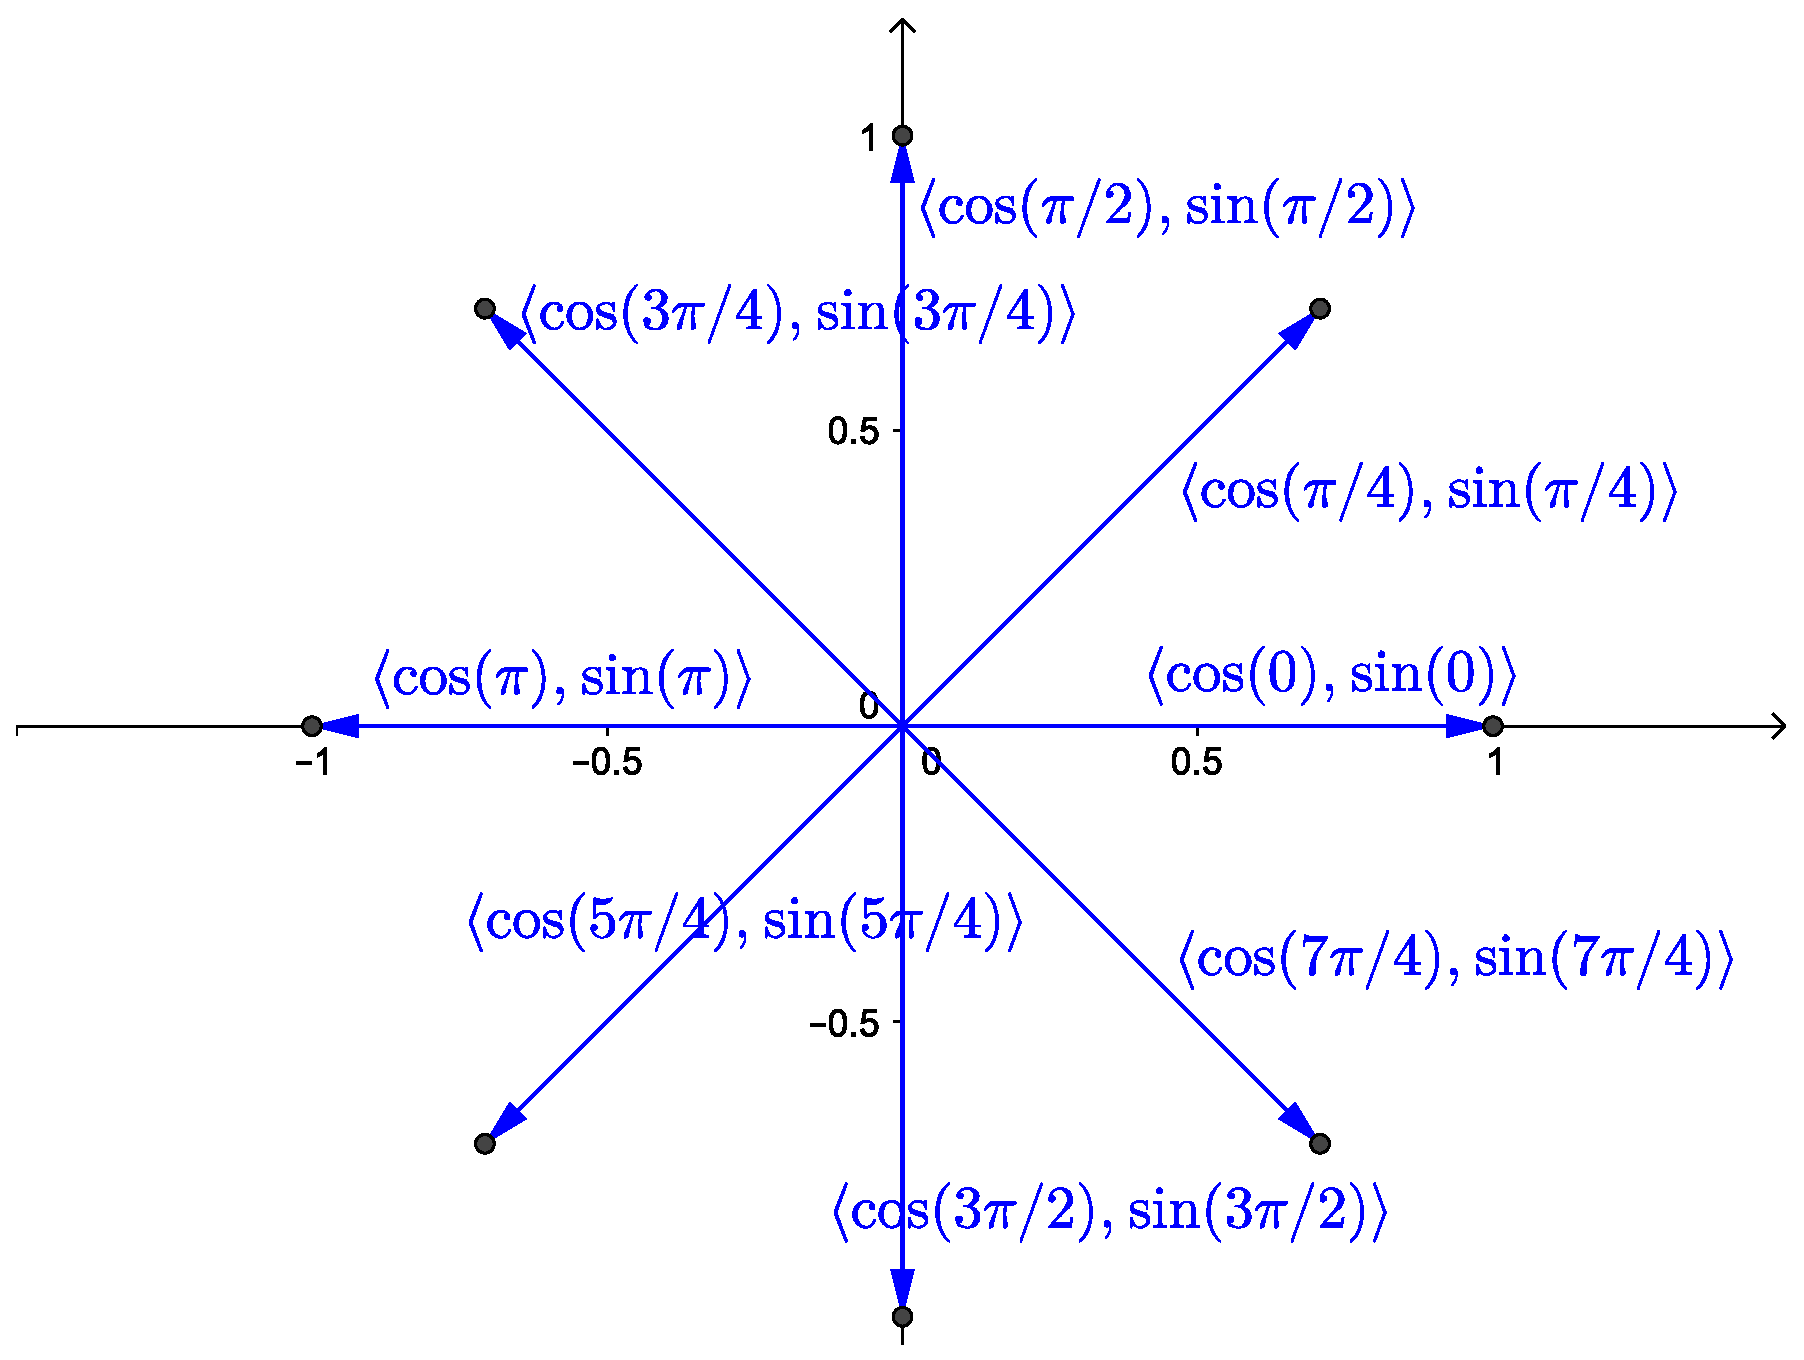
\includegraphics{figures/fig_9_6_PA_a.eps}} \resizebox{!}{2.5in}{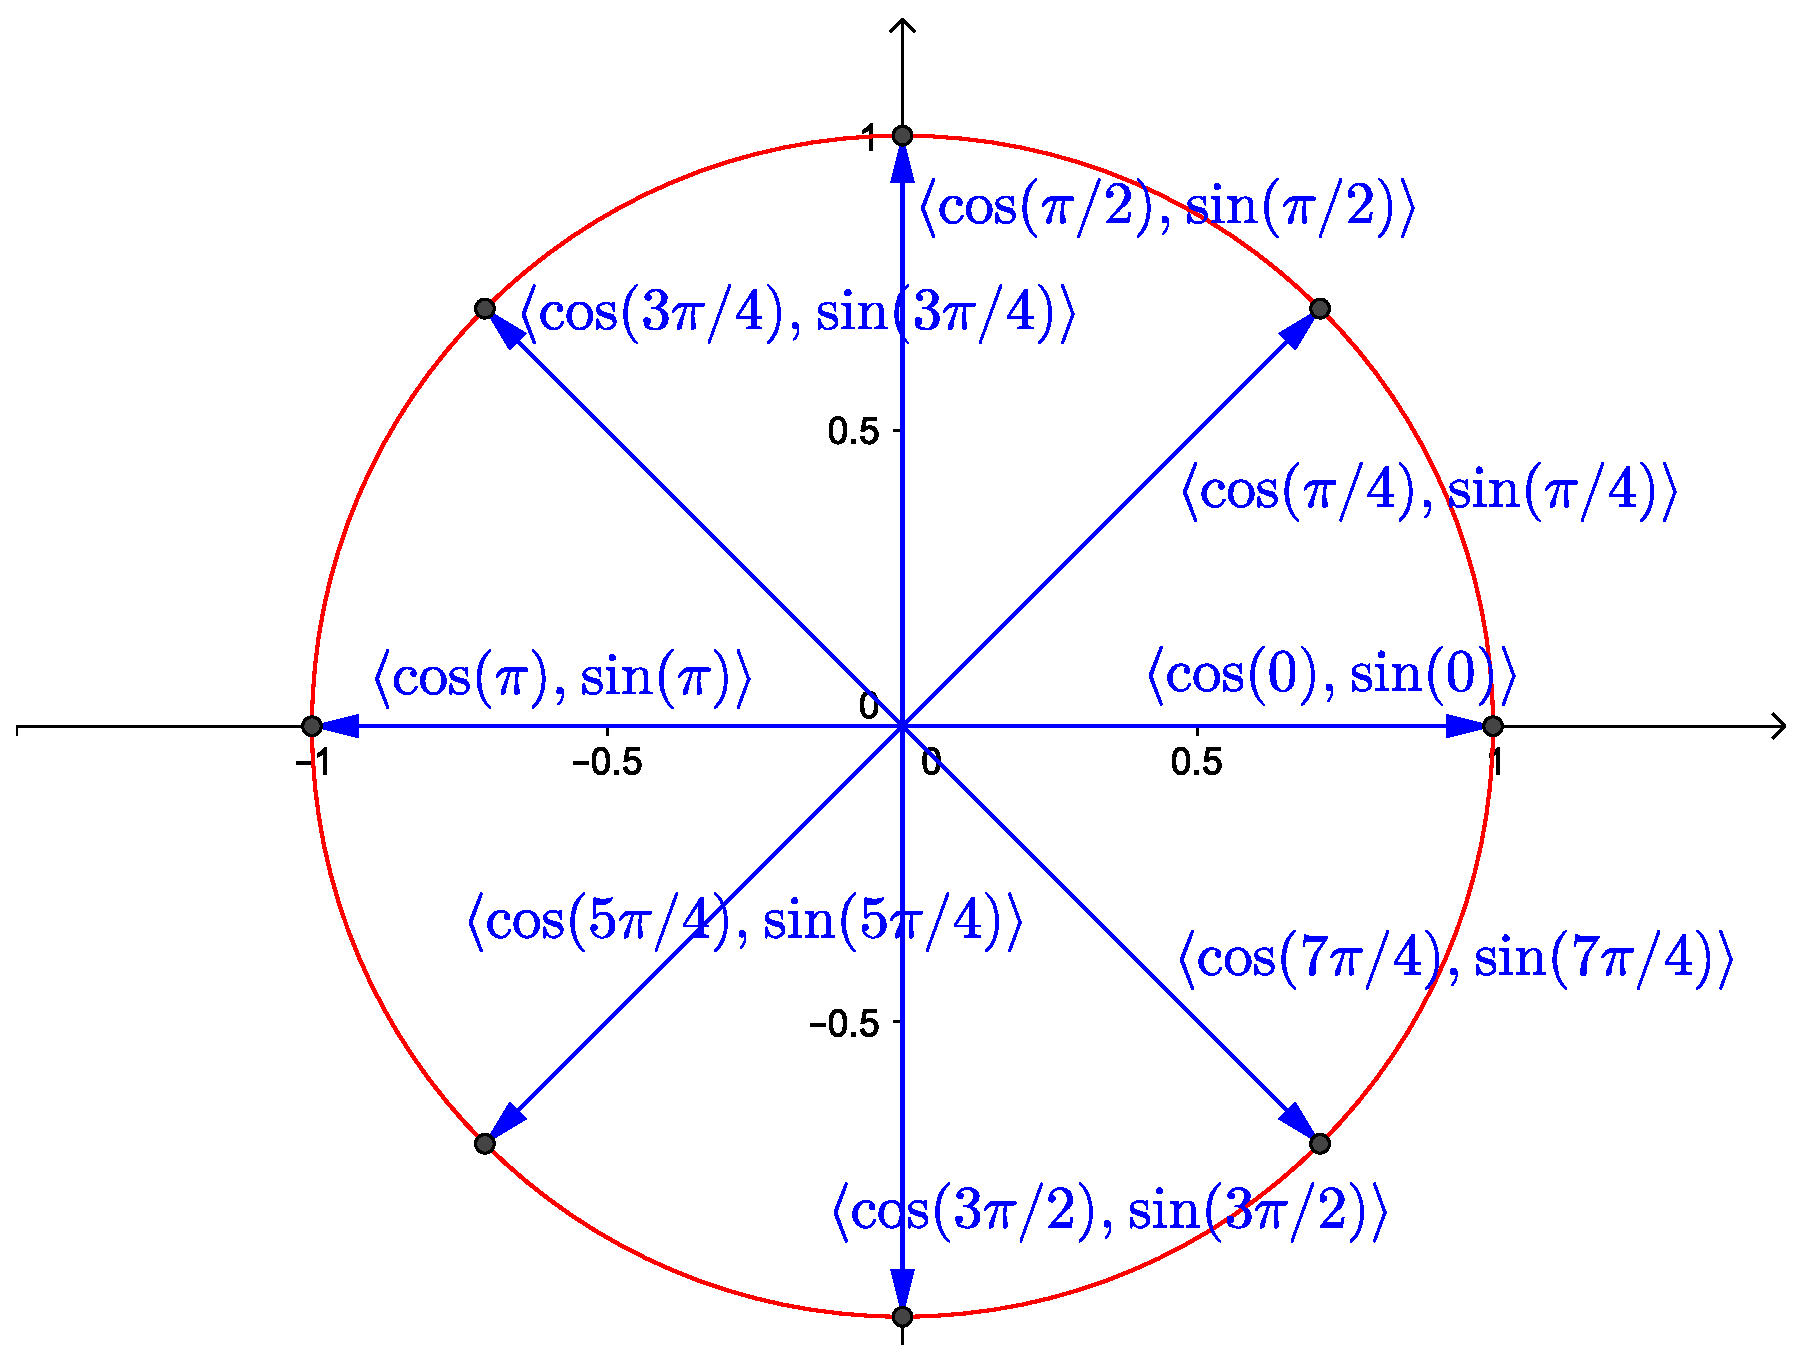
\includegraphics{figures/fig_9_6_PA_b.eps}}
  %       \caption{For part (f)}
 %       \label{F:9.3.preview.3}
      \end{center}
  %  \end{figure}
    

    \item The vectors are shown at left in the figure above. 


   \item The terminal points of these vectors all have the form $(\cos(t), \sin(t))$. Since $\cos^2(t) + \sin^2(t) = 1$, these points all lie on the unit circle as illustrated at right in the figure above.


    \ea
\end{activitySolution}

\afterpa 